На рисунке() представлена схема программируемой логики.\par 
\begin{figure}[ht]
    \centering
    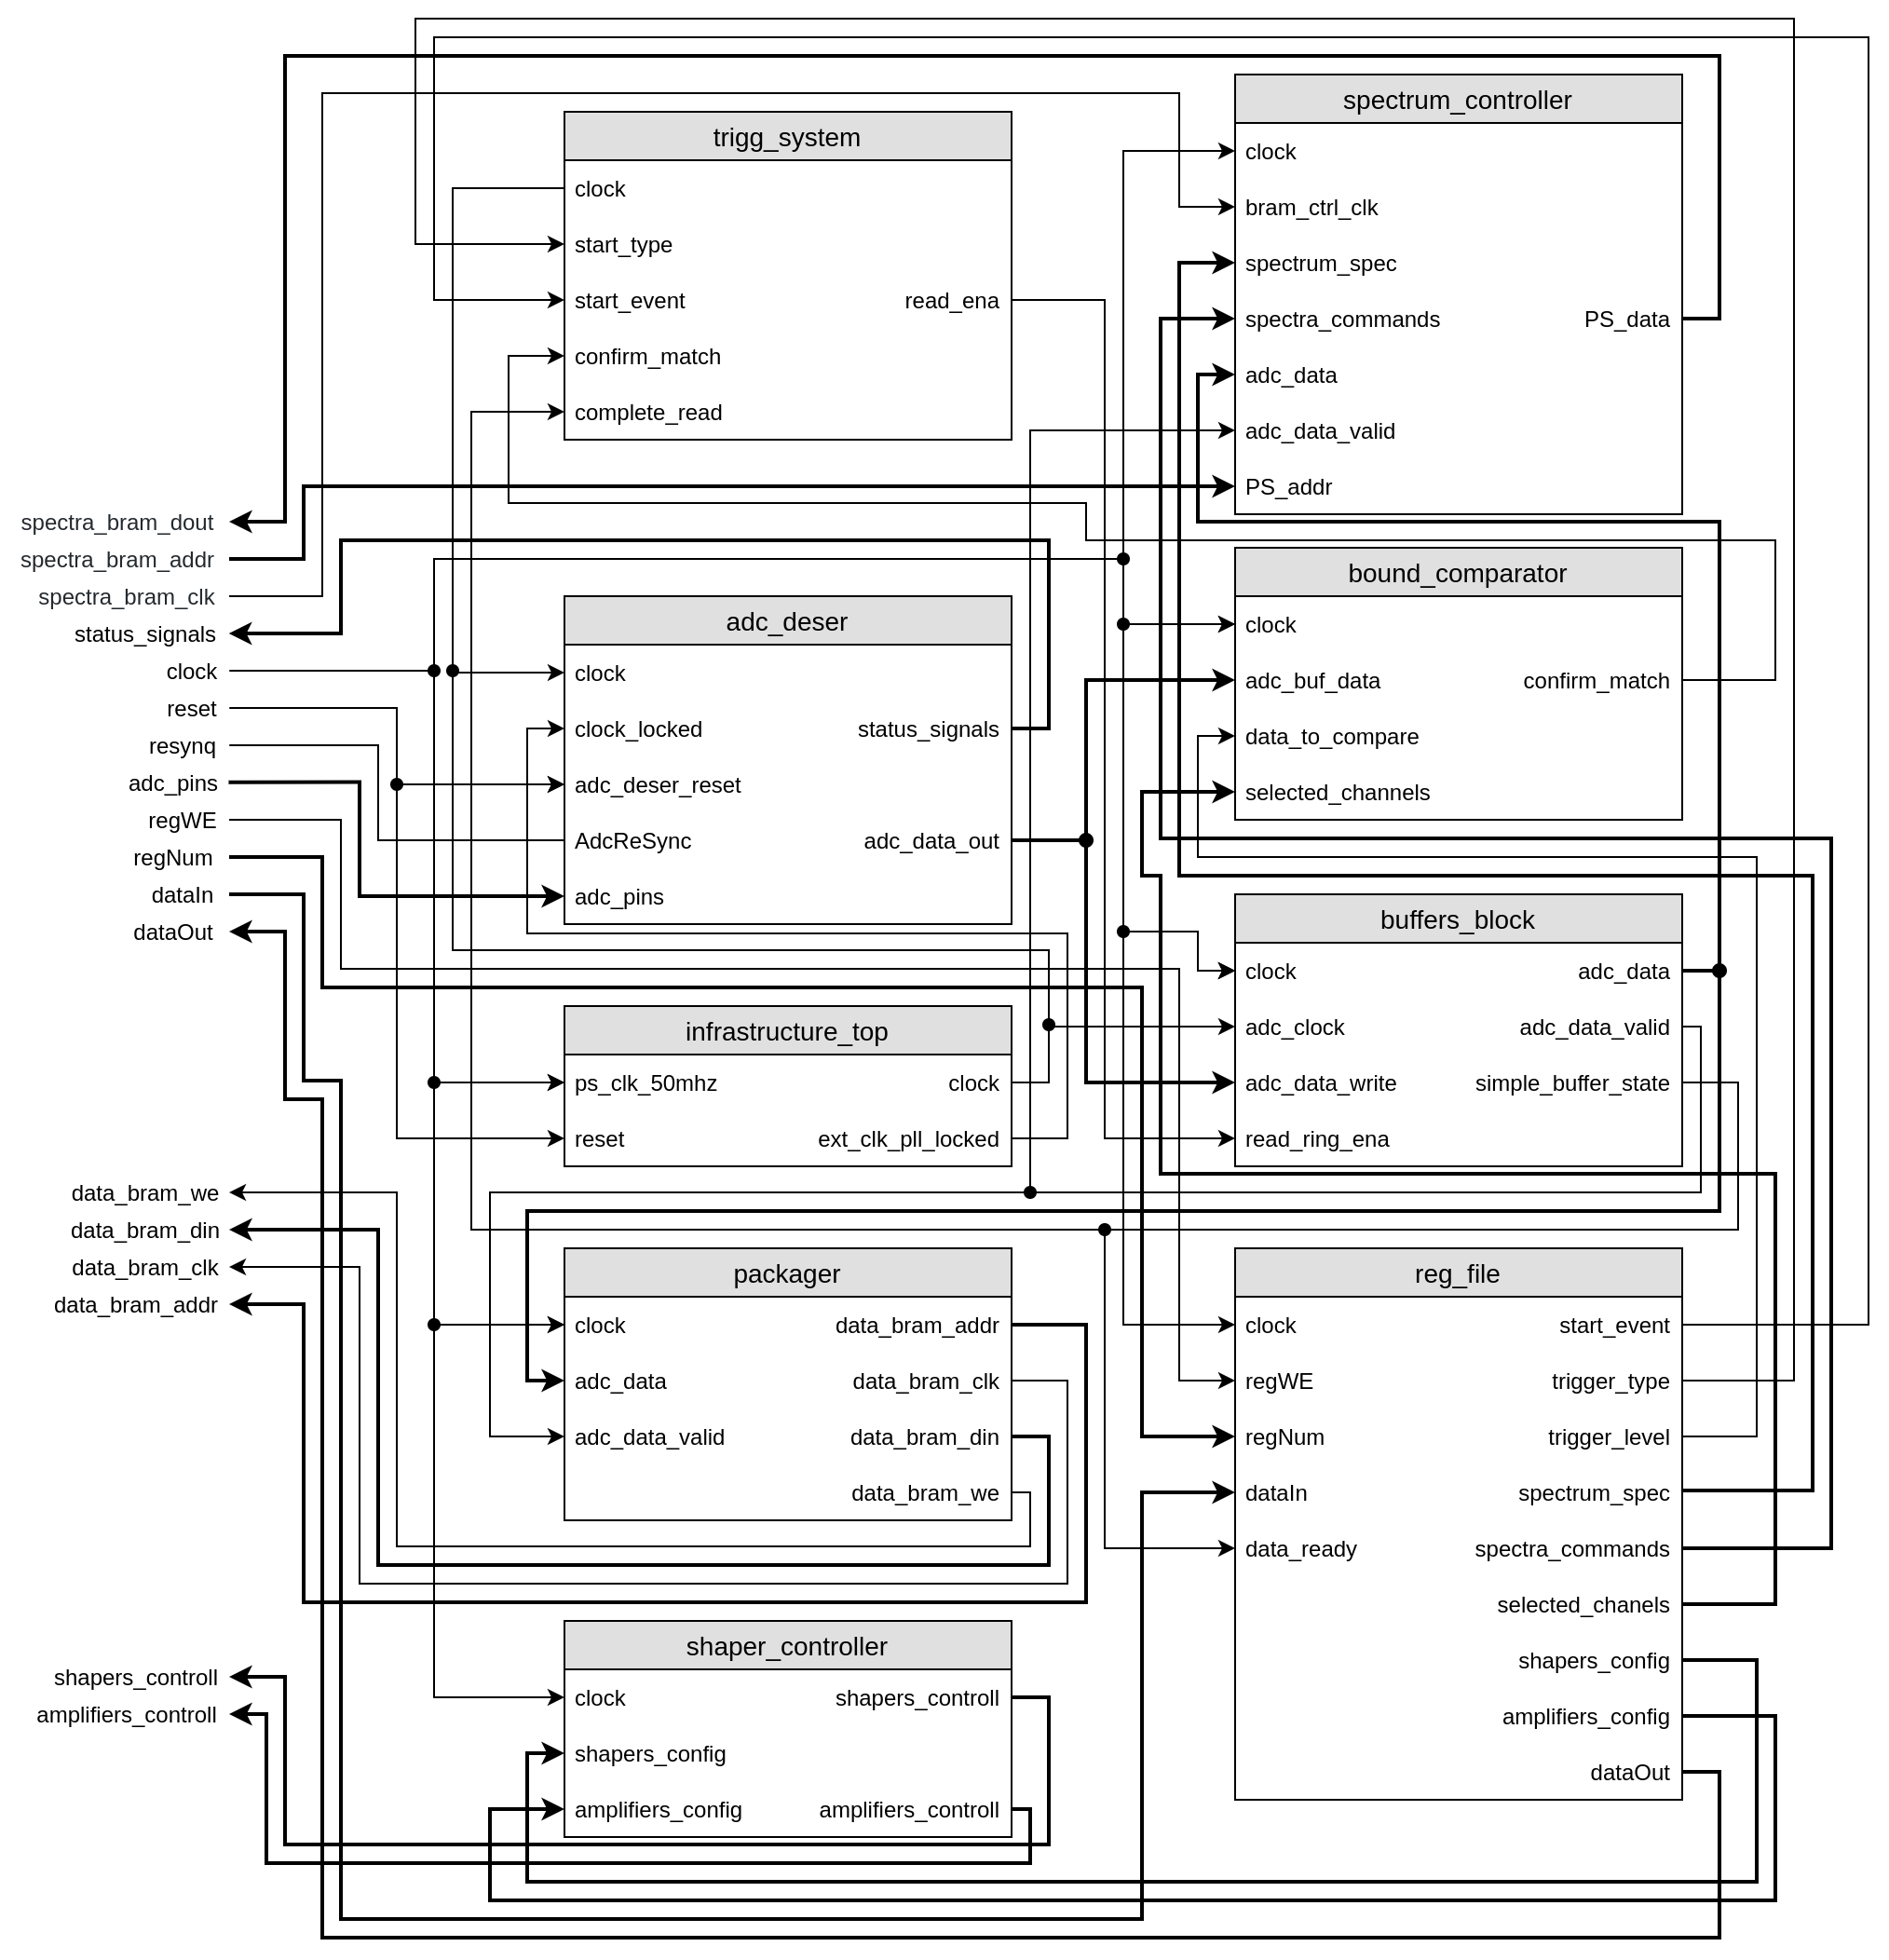
\includegraphics[width=1\linewidth]{PL_top.png}
    \caption{Блок-схема установки}
    \label{fig:mpr}
\end{figure}
Программируемая логика состоит из 9 блоков, краткое описание который представлено в таблице()\par
\begin{table}[h!]
    \caption{Блоки программируемой логики}
   % \begin{tabular}{|>{\centering\arraybackslash}p{0.45\textwidth}|>{\centering\arraybackslash}p{0.45\textwidth}|}
    \begin{tabular}{|p{0.45\textwidth}|p{0.5\textwidth}|}
        \hline
        Наименование блока & Описание \\
        \hline
        adc\_deser & Конвертирует упакованные последовательно данные АЦП в численные значения \\
        \hline
        infrastructure\_top & Обеспечивает тактовую частоту для некоторых модулей \\
        \hline
        buffers\_block & Буферизует входные данные \\
        \hline
        trigg\_system & Генерирует сигнал для сохранения данных \\
        \hline
        bound\_comparator & Выполняет сравнение входящих данных с заданными порогами \\
        \hline
        spectra\_controller & Производит обработку данных для набора статистики \\
        \hline
        shaper\_controller & Осуществляет управление формирователями сигналов \\
        \hline
        reg\_file & Реализует блок виртуальных регистров \\
        \hline
        packager & Упаковывает данные и передаёт их в процессорную систему \\
        \hline
    \end{tabular}
\end{table}
\textbf{Десериализатор adc\_deser}\par
Одним из основных элементов стенда является АЦП AD-9253. Данный преобразователь работает на 125 МГц параллельно в 4-х каналах. Данные с разрешением 14 бит передаются по протоколу LVDS. Данный стандарт предполагает передачу информации в последовательно-упакованном виде по 2 каналам на каждый вход. На рисунке() представлена временная диаграмма работы АЦП.\par
\begin{figure}[ht]
    \centering
    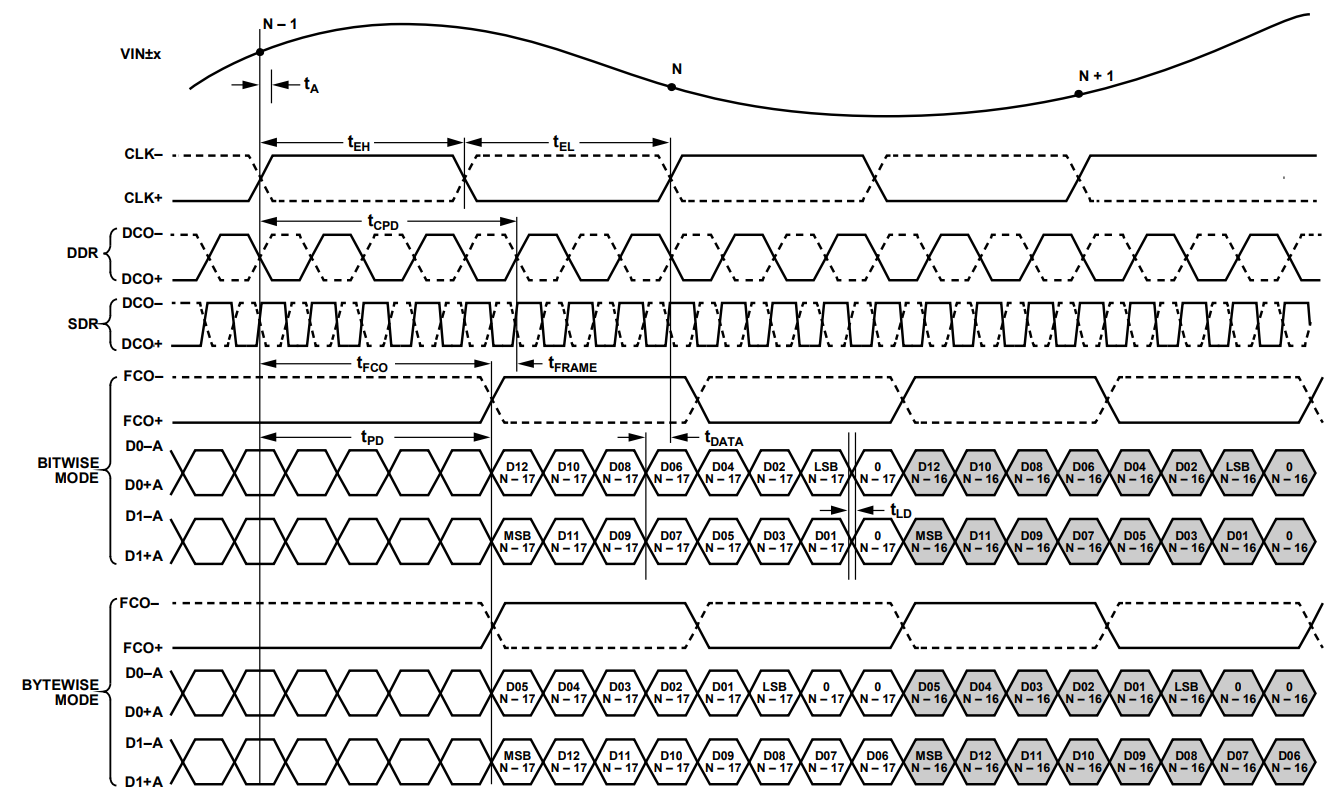
\includegraphics[width=1\linewidth]{ADC_time_diagram.png}
    \caption{Временная диаграмма работы АЦП}
    \label{fig:mpr}
\end{figure}
Каждый такт работы АЦП производится оцифровка входного аналогового сигнала. Как видно из временной диаграммы, полученные данные отправляются за 1 такт через 17 тактов после оцифровки по двум каналам. Предствляться они могут в одном из двух вариантов: побитовый (bitewise mode) и побайтовый (bytewise mode). Данные режимы отличаются последовательностью упаковки битов --- в разных каналах передаются либо четные и нечётные биты, либо младший и старший байты соответственно. В данной работе выбран побитовый режим, так как данные в таком виде проще обработать в программируемой логике.\par
Также в работе АЦП участвуют 2 вспомогательных сигнала --- кадровый, отвечающий за разделение набора бит на кадры оцифровки, и сигнал передачи данных, который размечает биты внутри каждого кадра.\par
Таким образом, возникает небходимость реализации модуля, осуществляющего конвертацию последовательности бит, поступающей из АЦП, в удобное для обработки численное значение. Так как процесс упаковки бит в определённую последовательность называется сериализацией, то обратную операцию можно назвать десериализаций, а соответствующий модуль --- десериализатором. Его сигналы изображены на рисунке()\par
\begin{figure}[ht]
    \centering
    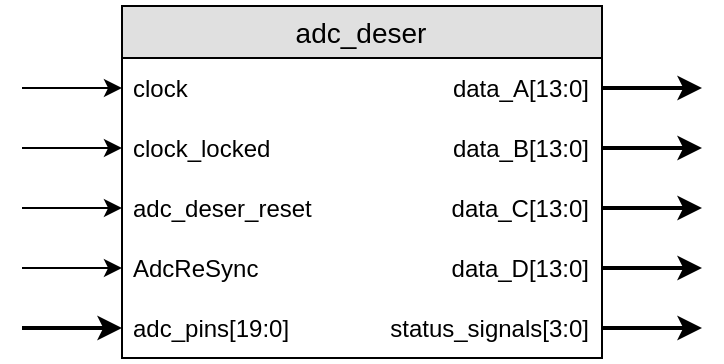
\includegraphics[width=0.5\linewidth]{adc_deser.png}
    \caption{Сигналы модуля десериализатора}
    \label{fig:mpr}
\end{figure}
Данный модуль был разработан ранее на основе готового интерфейса компании Xilinx, поэтому подробного описания его работы приведено не будет. Стоит лишь отметить, что входные данные принимаются через набор сигналов adc\_pins, а десериализованные значения подаются на выход через сигналы data\_i.\par
\textbf{ФАПЧ infrastructure\_top}\par
Модуль фазовой автоподстройки частоты (ФАПЧ) необходим для генерации тактового сигнала для работы АЦП и блоков, которые занимаются обработкой входных данных и их буферизацией (модули десериализатора и блока буферов). Как и десериализатор модуль ФАПЧ был разработан ранее с использованием библиотеки сложных функциональных блоков и рассматриваться подробно не будет. Сигналы модуля infrastructure\_top, в котором расположен ФАПЧ изображены на рисунке().\par
\begin{figure}[ht]
    \centering
    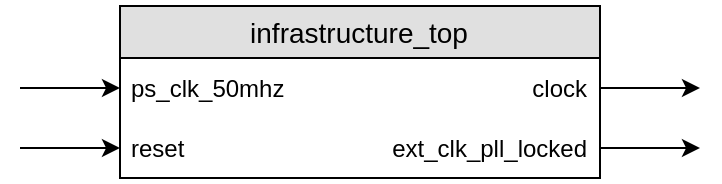
\includegraphics[width=0.5\linewidth]{infrastructure_top.png}
    \caption{Сигналы модуля infrastructure\_top}
    \label{fig:mpr}
\end{figure}
\textbf{Блок буферов buffers\_block}\par
В силу случайного характера возникновения полезных событий возникает необходимость временного хранения определённого числа последних измерений с АЦП. Для решения данной задачи был разработан модуль блока буферов, сигналы которого изображены на рисунке().\par
\begin{figure}[ht]
    \centering
    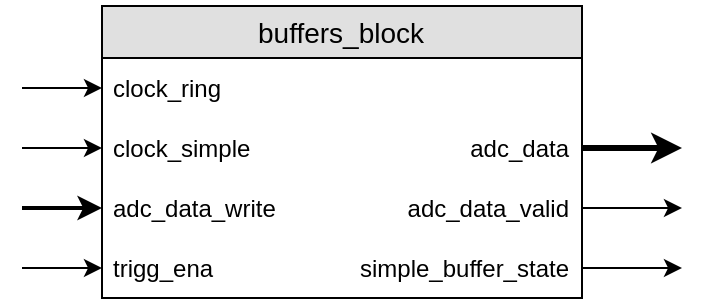
\includegraphics[width=0.5\linewidth]{buffers_block.png}
    \caption{Сигналы модуля блока буферов}
    \label{fig:mpr}
\end{figure}
Данный блок содежит в себе 2 модуля RAM памяти c раздельными портами чтения/записи данных. Первый является кольцевым буфером и непрерывно записывает данные с АЦП. Это позволяет сохранить некоторые данные до срабатывания триггерной системы. Такая необходимость обусловлена возможными задержками сигнала триггера, а также потербностью иметь небольшую "предысторию" осциллограммы перед достижением сигнала порогового значения.\par
Второй модуль памяти выполняет функцию простого буфера, в который временно будут выгружаться полезные данные при возникновении сигнала триггерной системы. Главной задачей такого буфера является хранение данных для гарантированного считывания и передачи их в процессорную систему.\par
Объём простого буфера определяется необходимым размером осциллограммы, который, в свою очередь, зависит от максимального времени высвечивания кристалла. Данное время ограничено промежутком в 1 мкс, следовательно, учитывая частоту работы АЦП (105 Мгц), требуемый размер буфера составляет порядка 100 кадров. Для удобства объём был увеличен до 128 -- осциллограмма будет подробнее, а адресация внутри буфера проще. Объём кольцевого буфера, в свою очередь, определяется максимальным колличеством данных, необходимого для восстановления. Из свойств сцинтилляционных кристаллов было принято решение, что 64 кадров будет хватать с запасом.\par
Модуль buffers\_block имеет два входных тактовых сигнала -- clock\_ring и clock\_simple. Система на кристалле работает на 50 МГц, следовательно именно на этой частоте должны выгружаться данные в процессорную часть. При этом АЦП работает на 105 МГц. Здесь кроется ещё одна немаловажная задача простого буфера: переход работы с данными с одной тактовой частоты на другую. Таким образом, поток данных поступает в блок на тактовом сигнале работы АЦП, а полезная информация выдаётся на частоте работы системы на кристалле.\par
Из рисунка видно, что модуль также содержит следующие входные сигналы: adc\_data\_write -- входные данные с АЦП, trigg\_ena -- сигнал триггерной системы о возникновении полезного события. Также можно заметить, что выходной набор adc\_data содержит большее число сигналов, чем входной adc\_data\_write. Это связано с добавлением к данным по 2 бита, индетифицирующих их отношение к определённому каналу. Таким образом, значение каждой оцифровки хранится ровно в двух байтах.\par
\textbf{Триггерная система trigg\_system}\par
Как было сказано ранее, для сохранения данных с АЦП в буфер и последующей их передачи в процессор необходим сигнал, сообщающий о возникновении полезного события. Генерацией такого сигнала занимается модуль триггерной системы, сигналы которого изображены на рисунке().\par
\begin{figure}[ht]
    \centering
    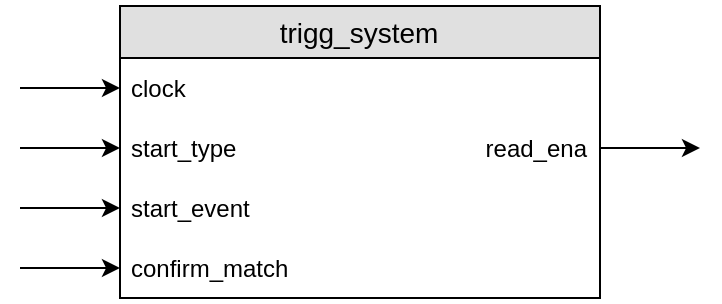
\includegraphics[width=0.5\linewidth]{trigg_system.png}
    \caption{Сигналы модуля триггерной системы}
    \label{fig:mpr}
\end{figure}
Триггерная система может работать в двух режимах, которые задаются сигналом start\_type: принудительно и по порогу. В первом случае модуль отработает сразу при появлении сигнала старта на входе start\_event. В режиме срабатывания по порогу триггер сгенерирует разрешение на запись только при появлении на входе confirm\_match высокого уровня от модуля компаратора bound\_comparator.\par
\textbf{Компаратор bound\_comparator}\par
Компаратор осуществляет сравнение текущих оцифрованных данных АЦП с заданными оператором значениями порогов. Это необходимо для корректного функционирования триггерной системы в соответствующем режиме работы. Сигналы данного блока изображены на рисунке()\par
\begin{figure}[ht]
    \centering
    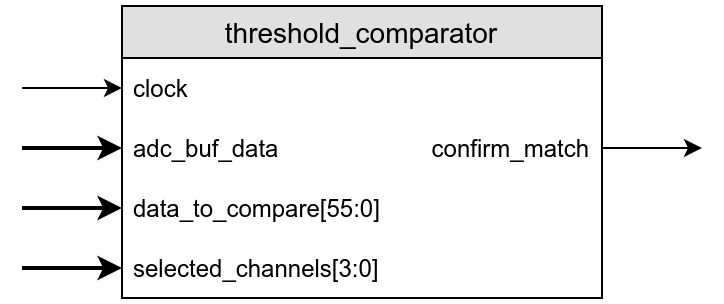
\includegraphics[width=0.5\linewidth]{bound_comparator.png}
    \caption{Сигналы модуля компаратора}
    \label{fig:mpr}
\end{figure}
Данный модуль функционирует на тактовой частоте работы АЦП, т.к. он должен непрерывно сравнивать каждое оцифрованное значение, поступающее через вход adc\_buf\_data. При достижении или превышении порогового значения модуль формирует на выходном сигнале confirm\_match логическую единицу и ноль в противоположном случае. Порог для каждого канала задаётся отдельно с помощью сигналов data\_to\_compare. Стоит отметить, что реализована возможность выбирать каналы, выполнение условий по которым повлечёт срабатывание модуля. Оператор может назначать их в режиме логического ИЛИ: система выдаст сигнал при срабатывании компаратора хотя бы по одному из выбранных каналов. Эта информация поступает в блок компаратора через сигналы selected\_channels.\par
\textbf{Модуль набора статистики spectra\_controller}\par
\textbf{Управление блоком формирователей shapers\_controller}\par
\textbf{Модуль виртуальных регистров reg\_file}\par
\textbf{Упаковщик packager}\par
